\documentclass{article}\usepackage[]{graphicx}\usepackage[]{color}
%% maxwidth is the original width if it is less than linewidth
%% otherwise use linewidth (to make sure the graphics do not exceed the margin)
\makeatletter
\def\maxwidth{ %
  \ifdim\Gin@nat@width>\linewidth
    \linewidth
  \else
    \Gin@nat@width
  \fi
}
\makeatother

\definecolor{fgcolor}{rgb}{0.345, 0.345, 0.345}
\newcommand{\hlnum}[1]{\textcolor[rgb]{0.686,0.059,0.569}{#1}}%
\newcommand{\hlstr}[1]{\textcolor[rgb]{0.192,0.494,0.8}{#1}}%
\newcommand{\hlcom}[1]{\textcolor[rgb]{0.678,0.584,0.686}{\textit{#1}}}%
\newcommand{\hlopt}[1]{\textcolor[rgb]{0,0,0}{#1}}%
\newcommand{\hlstd}[1]{\textcolor[rgb]{0.345,0.345,0.345}{#1}}%
\newcommand{\hlkwa}[1]{\textcolor[rgb]{0.161,0.373,0.58}{\textbf{#1}}}%
\newcommand{\hlkwb}[1]{\textcolor[rgb]{0.69,0.353,0.396}{#1}}%
\newcommand{\hlkwc}[1]{\textcolor[rgb]{0.333,0.667,0.333}{#1}}%
\newcommand{\hlkwd}[1]{\textcolor[rgb]{0.737,0.353,0.396}{\textbf{#1}}}%

\usepackage{framed}
\makeatletter
\newenvironment{kframe}{%
 \def\at@end@of@kframe{}%
 \ifinner\ifhmode%
  \def\at@end@of@kframe{\end{minipage}}%
  \begin{minipage}{\columnwidth}%
 \fi\fi%
 \def\FrameCommand##1{\hskip\@totalleftmargin \hskip-\fboxsep
 \colorbox{shadecolor}{##1}\hskip-\fboxsep
     % There is no \\@totalrightmargin, so:
     \hskip-\linewidth \hskip-\@totalleftmargin \hskip\columnwidth}%
 \MakeFramed {\advance\hsize-\width
   \@totalleftmargin\z@ \linewidth\hsize
   \@setminipage}}%
 {\par\unskip\endMakeFramed%
 \at@end@of@kframe}
\makeatother

\definecolor{shadecolor}{rgb}{.97, .97, .97}
\definecolor{messagecolor}{rgb}{0, 0, 0}
\definecolor{warningcolor}{rgb}{1, 0, 1}
\definecolor{errorcolor}{rgb}{1, 0, 0}
\newenvironment{knitrout}{}{} % an empty environment to be redefined in TeX

\usepackage{alltt}
\usepackage{amscd, amssymb, amsmath, verbatim, setspace}
\usepackage[left=1.0in, right=1.0in, top=1.0in, bottom=1.0in]{geometry}
\usepackage{mathrsfs}
\usepackage{listings}


\IfFileExists{upquote.sty}{\usepackage{upquote}}{}
\begin{document}
\begin{flushright}
  Arif Ali\\
  ANLY-511 Prob. Modeling \& Stat. Computing\\
	Nov 20, 2015\\
\end{flushright}

\begin{center}
  \LARGE\textbf{Homework \#9}
\end{center}
\section*{Exercise 65}
\begin{knitrout}
\definecolor{shadecolor}{rgb}{1, 1, 1}\color{fgcolor}\begin{kframe}
\begin{verbatim}
set.seed(1212331312)
Titanic = read.csv("~/Dropbox/School/Georgetown/Analytics 511 Fall 2015/ChiharaHesterberg/Titanic.csv")
Titanic_dead = Titanic$Age[Titanic$Survived==0]
Titanic_alive = Titanic$Age[Titanic$Survived==1]

bootstrap_Titanic_dead = replicate(10000, median(sample(Titanic_dead, length(Titanic_dead), replace = T)))
bootstrap_Titanic_alive = replicate(10000, median(sample(Titanic_alive, length(Titanic_alive), replace = T)))

quantile(bootstrap_Titanic_alive - 
           bootstrap_Titanic_dead, 
         c(0.05, 0.95))
##  5% 95% 
##  -4   1
\end{verbatim}
\end{kframe}
\end{knitrout}
I created a $90\%$ confidence interval in order to see if 0 is within the interval. Based on the confidence interval, I'm $90\%$ confident that the difference between the bootstrap medians is betwwen -4 and 1.

\section*{Exercise 66}
\begin{knitrout}
\definecolor{shadecolor}{rgb}{1, 1, 1}\color{fgcolor}\begin{kframe}
\begin{verbatim}
loglikeli.exp = function(lambda,x){log(lambda^(length(x))*exp(-lambda*sum(x)))}
# Note: by log properties this could alos have been length(x)*log(lambda) - lambda*sum(x)
t = seq(.01,5,by = .01)
y = c()
x1 <- rexp(5,rate = 2)
for (j in 1:500) y[j] <- loglikeli.exp(t[j],x1)
plot(t,y, xlab = 'lambda', ylab = 'likelihood')
\end{verbatim}
\end{kframe}
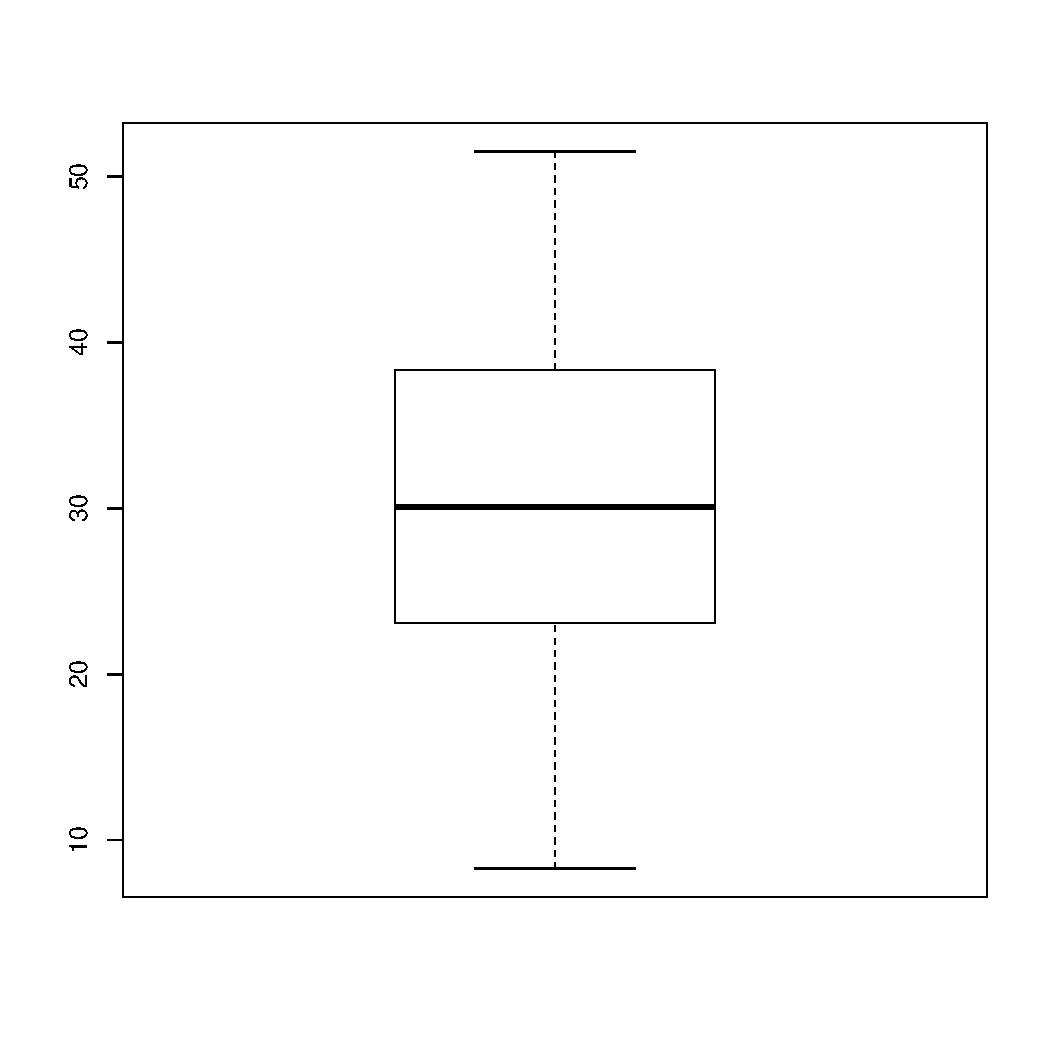
\includegraphics[width=0.33\linewidth]{figure/unnamed-chunk-3-1} 
\begin{kframe}\begin{verbatim}
t[y==max(y)]
## [1] 1.51
\end{verbatim}
\end{kframe}
\end{knitrout}
It's interesting to see that the maximum value is actually occuring before the value of, around the value of 2, but never exactly at. Please note, I did not use 
\section*{Exercise 70}
\begin{knitrout}
\definecolor{shadecolor}{rgb}{1, 1, 1}\color{fgcolor}\begin{kframe}
\begin{verbatim}
set.seed(301323)
likelihood.cauchy = function(x, theta){
  return((prod(pi*(1+(x-theta)^2)))^-1)
}

t = seq(-30,30,by = .01)
y = c()
x1 <- rcauchy(4)
for (j in 1:length(t)) y[j] <- likelihood.cauchy(x1,t[j])
plot(t,y, xlab = 'theta', ylab = 'likelihood')
\end{verbatim}
\end{kframe}
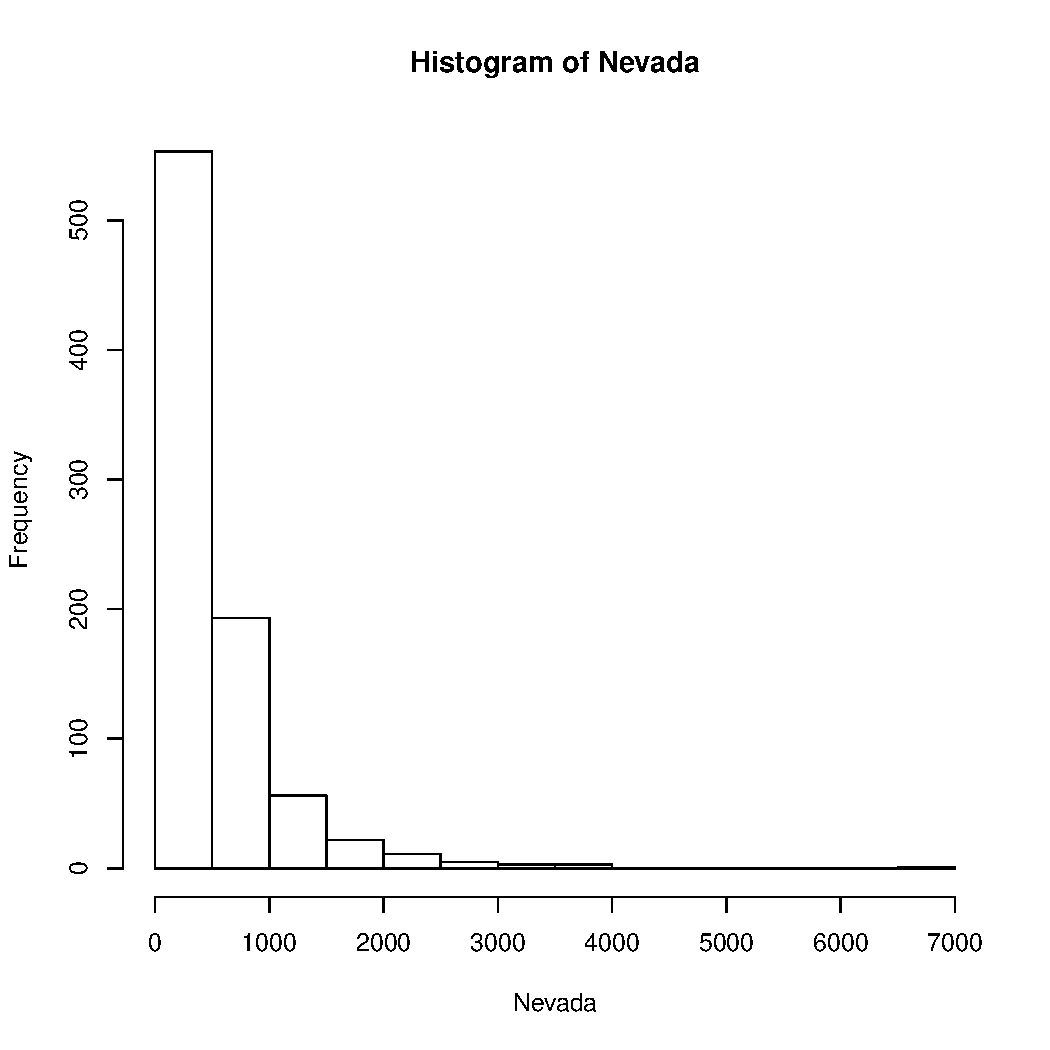
\includegraphics[width=0.33\linewidth]{figure/unnamed-chunk-4-1} 
\begin{kframe}\begin{verbatim}
x1 <- rcauchy(2)
for (j in 1:length(t)) y[j] <- likelihood.cauchy(x1,t[j])
plot(t,y, xlab = 'theta', ylab = 'likelihood')
\end{verbatim}
\end{kframe}
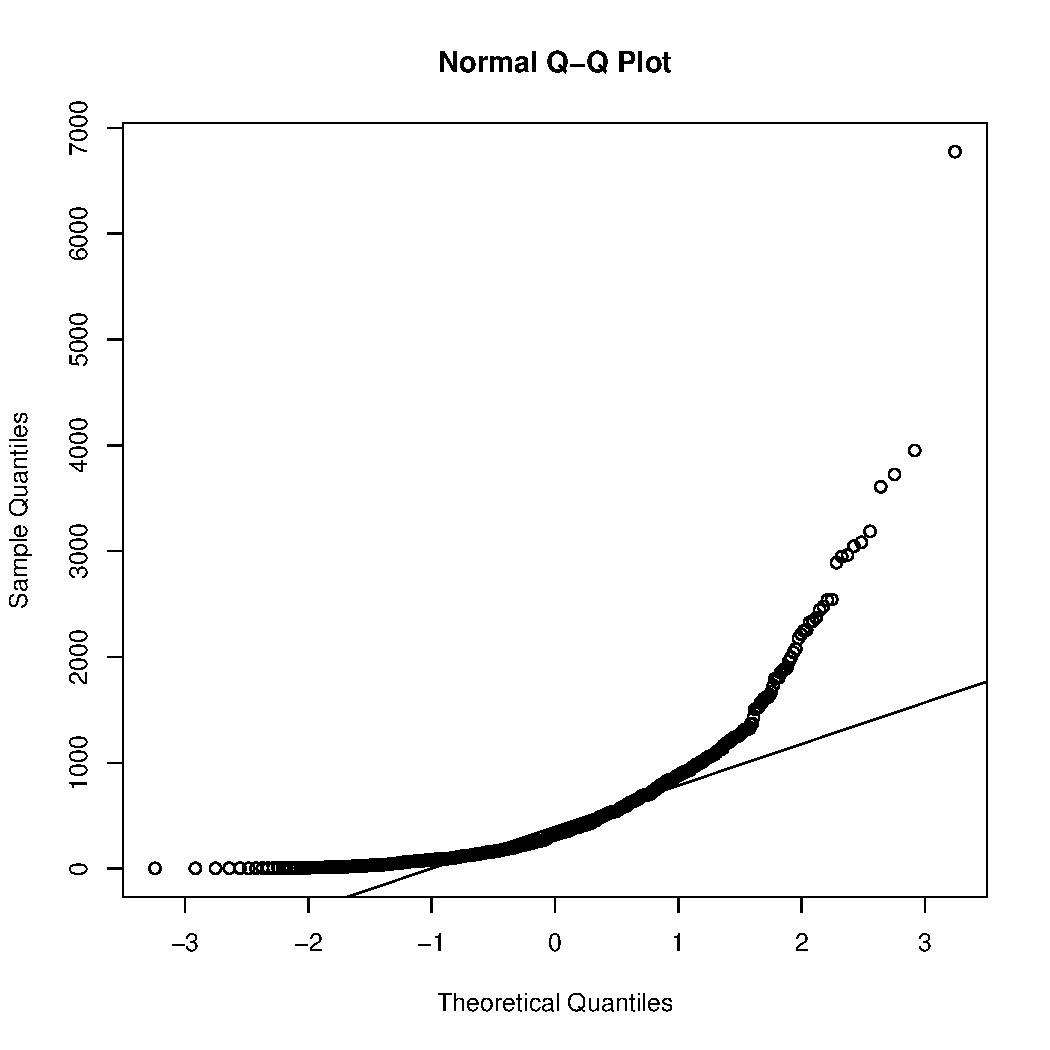
\includegraphics[width=0.33\linewidth]{figure/unnamed-chunk-4-2} 

\end{knitrout}
At $n=10$, it seems like that there is always one local maximum values. At $n=4$, there two local maximums can be observed a few (but not a majority of) times; It didn't occur at the set seed. When lowering n to 2, the number of maximums seems to be greater than 1 at a more frequent rate, as observed by the graph. Looking at the varying sample sizes, it seems clear that in order to best fine tune a MLE value, we should increase the sample size.   
\section*{Exercise 71}
\begin{knitrout}
\definecolor{shadecolor}{rgb}{1, 1, 1}\color{fgcolor}\begin{kframe}
\begin{verbatim}
rcauchy.fun = function(n){
  x1 <- rcauchy(n)
  return(
    c(abs(mean(x1, trim = 0.1)),
             abs(median(x1))))
}
sample.sizes = c(10,20,40,100)

ab = matrix(nrow = length(sample.sizes), ncol = 2)
for(n in 1:length(sample.sizes)){
    print(paste0(c("The size of sample is",n)))
    aa = t(replicate(10000, rcauchy.fun(sample.sizes[n])))
    ab[n, 1] = var(aa[,1])
    ab[n, 2] = var(aa[,2])
}
## [1] "The size of sample is" "1"                    
## [1] "The size of sample is" "2"                    
## [1] "The size of sample is" "3"                    
## [1] "The size of sample is" "4"
ab
##            [,1]        [,2]
## [1,] 1.72017676 0.157327131
## [2,] 0.54498698 0.055367059
## [3,] 0.06050877 0.024901495
## [4,] 0.01967146 0.009403356
\end{verbatim}
\end{kframe}
\end{knitrout}
For each of the sample sizes the variance median is more smaller compared to the variance of the trimmed mean. However, as the sample size increases the variance of the median decreases. Thus, the efficiency seems to be dependent in relation to size. As size goes up, the variance of the median goes down, meaning that efficiency is increasing.

\section*{Additional Exercises}
Please see next page
\end{document}
